\documentclass{beamer}
\beamertemplatenavigationsymbolsempty
\usecolortheme{beaver}
\setbeamertemplate{blocks}[rounded=true, shadow=true]
\setbeamertemplate{footline}[page number]
%
\usepackage[utf8]{inputenc}
\usepackage[english,russian]{babel}
\usepackage{amssymb,amsfonts,amsmath,mathtext}
\usepackage{subfig}
\usepackage[all]{xy} % xy package for diagrams
\usepackage{array}
\usepackage{multicol}% many columns in slide
\usepackage{hyperref}% urls
\usepackage{hhline}%tables
% Your figures are here:
\graphicspath{ {fig/} {../fig/} }

%----------------------------------------------------------------------------------------------------------
\title[\hbox to 56mm{Задачи планирования}]{	Экспериментальное сравнение \\ задач оперативного планирования биохимического производства}
\author[В.\,В. Пырэу]{Виталий Вячеславович Пырэу}
\institute{Московский физико-технический институт}
\date{\footnotesize
\par\smallskip\emph{Курс:} Автоматизация научных исследований\par (практика, В.\,В.~Стрижов)/Группа Б05-821
\par\smallskip\emph{Эксперт:} С.\,А.~Тренин
\par\bigskip\small 2021}
%----------------------------------------------------------------------------------------------------------
\begin{document}
%----------------------------------------------------------------------------------------------------------
\begin{frame}
\thispagestyle{empty}
\maketitle
\end{frame}

\begin{frame}{Моделирование расписания для производства}
\textbf{Основная решаемая задача}: получить оптимальное или качественное допустимое расписание для производства, используя как можно более простую модель.

\bigskip

\textbf{Цель исследования}: сравнить дискретный и непрерывный подходы к моделированию расписаний и описать классы задач, в которых модели, полученные в рамках каждого из подходов будут проще.

\bigskip

\textbf{Критерии качества}: число переменных и ограничений модели, производящей расписание для различных процессов
\end{frame}

\begin{frame}{Постановка практической задачи}
\begin{enumerate}
	\item Известны рецепты промежуточных прекурсоров и продуктов производства (в виде STN диаграммы).
	\item Известны длительности промежуточных работ
	\item Известны параметры производственных узлов и складов завода.
	\item Известны количество материала в момент начала производства и требования на продукт.
\end{enumerate}
\begin{center}
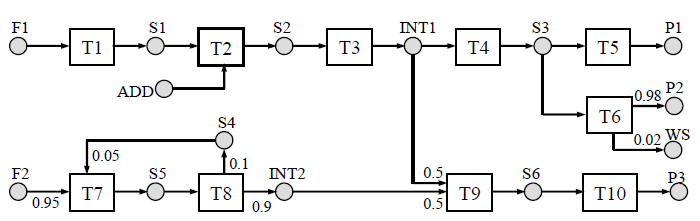
\includegraphics[width=1.0\textwidth]{stagedstn}
\end{center}
\end{frame}

\begin{frame}{Подходы к моделированию требований к расписанию}
\begin{enumerate}
	\item Практические требования моделируются как задачи ЦЛП в общей форме
	\item Индикаторы начала и конца работы в заданный момент времени 
	\item Использование прореженной сетки с последующим сдвигом расписания влево (двухступенчатая схема)
	\item Индикаторы порядка на событиях начала и конца работы (схема порядка)
\end{enumerate}

\end{frame}

\begin{frame}{Литература}
	\begin{enumerate}
	\item \textbf{STN-диаграммы}: E. Kondili, С. C. Pantelidest and R. W. H. Sargent. A general algorithm for short-term scheduling of batch operations-i. MILP formulation
	\item \textbf{Обзор современных достижений}: Georgios P. Georgiadis, Apostolos P. Elekidis and Michael C. Georgiadis. Optimization-based scheduling for the process Industries: from theory to real-life Industrial applications.
	\item \textbf{Двухступенчатая схема}: F. Blomer, H.-O. Gunther. LP-based heuristics for scheduling chemical batch processes.
	\item \textbf{Схема, основанная на порядке}: C.A. Mendez, G.P. Henning, J. Cerda. An MILP continuous-time approach to short-term scheduling of resource-constrained multistage flowshop batch facilities.
\end{enumerate}
\end{frame}

\begin{frame}{Требование к расписанию}
	Расписание должно быть оптимальным с точки зрения целевой функции - Makespan и учитывать следующие ограничения:
	\begin{enumerate}
	\item На конец производства выполнен весь заказ, то есть произведено как минимум столько продукта, сколько требовалось
	\item Склад не переполнен в течении всего времени производства
	\item Всякий процесс в расписании может взять со склада требуемый ему материал
	\item Один узел в каждый момент времени занимается не более, чем одной задачей
\end{enumerate}
\end{frame}

\begin{frame}{Дискретная модель с плотным временем}
	\begin{enumerate}
	\item Переменные-индикаторы того, что процесс берёт задачу в некоторый момент
	\item Поток материала в каждый момент времени --- взвешанная сумма индикаторов
	\item Гарантируется получение оптимального расписания
	\item С удлинением временной шкалы число переменных резко возрастает даже при небольшом числе задач.
\end{enumerate}

\begin{center}
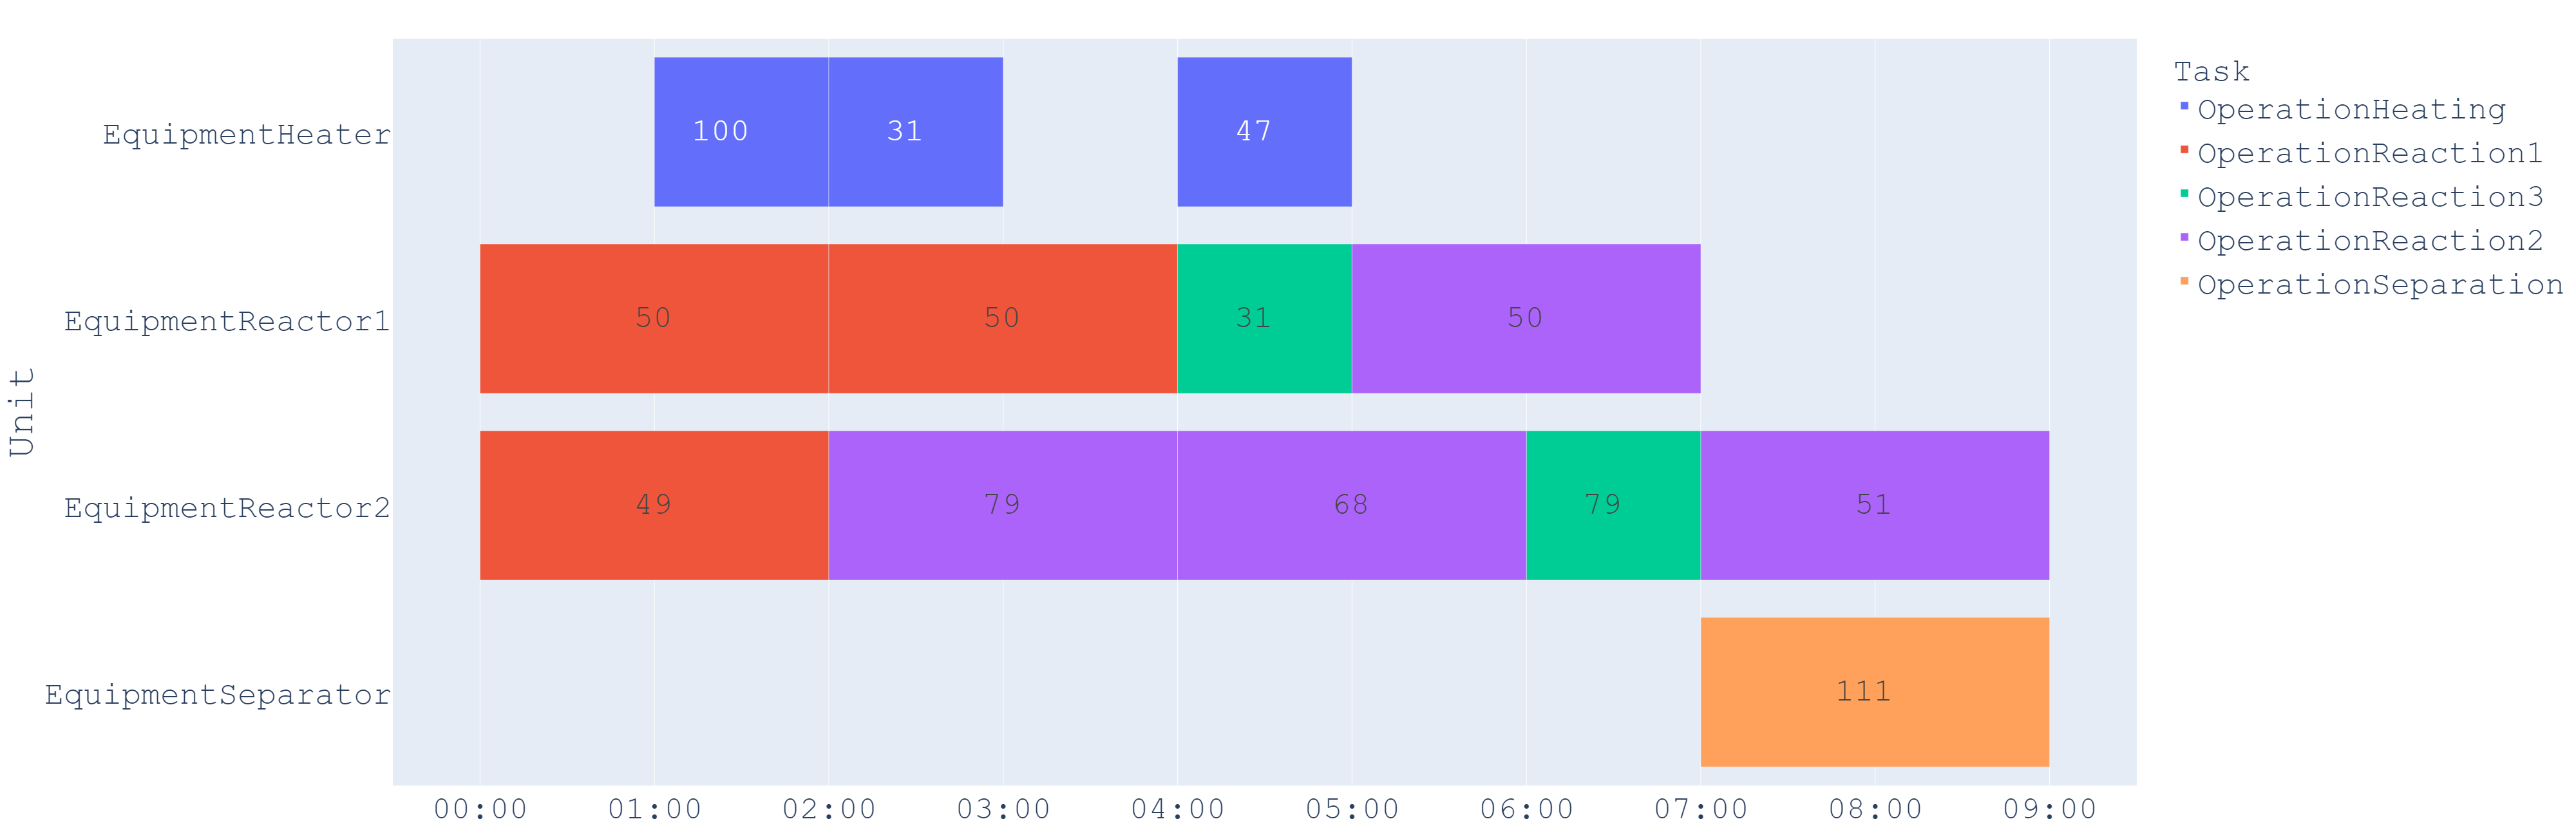
\includegraphics[width=1.0\textwidth]{plan}
\end{center}

\end{frame}

\begin{frame}{Двухступенчатая схема}
	\begin{enumerate}
	\item Решает проблему длинной временной шкалы
	\item Делит получение расписания на две фазы: грубое приближение и уточнение
	\item На первой фазе задачам разрешено начинаться только в малое число точек времени
	\item Не гарантирует получение оптимального расписания, но даёт качественные практичные приближения.
	\item Подбор разряженности временной шкалы позволяет настроить степень сложности модели и оптимальности получаемого расписания
\end{enumerate}

\begin{center}
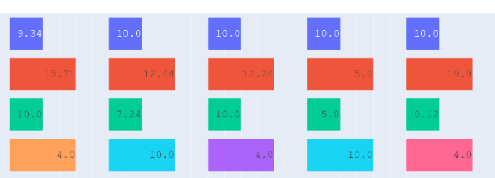
\includegraphics[width=0.85\textwidth]{plan sparsed}
\end{center}

\end{frame}

\begin{frame}{Схема, основанная на порядке}
	\begin{enumerate}
	\item Минимально моделирует временную шкалу
	\item Берёт во внимание не точное время событий, а их очерёдность
	\item Число переменных растёт квадратично от числа задач, но не зависит от плотности временной шкалы.
	\item Модели становятся более сложными, если процесс сетевой и простыми, если процесс линейный.
	
\begin{center}
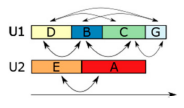
\includegraphics[width=0.85\textwidth]{precendance model}
\end{center}
	
\end{enumerate}


\end{frame}

\begin{frame}{Итоги эксперимента по моделированию расписаний}

\fontsize{10pt}{20pt}
\selectfont
\centering
\renewcommand{\arraystretch}{2}
	\resizebox{\columnwidth}{!}{\begin{tabular}{ |c|c|c|c|c| }
		 \hline
		 Процесс/модель & Дискретная & Двухступенчатая & Порядковая \\ [2ex] 
		 \hline\hline
		 Demand 500, время 50, простой сетевой процесс & 1276/1859 & 276+1471/379+1589  & 41431/121494  \\ 
		 \hline
		 Demand 50, время 10, простой сетевой процесс & 276/379 & 151+829/194+854& 1735/5070   \\
		 \hline
		 Модельный немецкий пример, время 120 & 8108/12019  & 1408+26965/2019+32276 & 37761/106801   \\
		 \hline
		 Поэтапный процесс, время & 4115/6014 & 1735+72749/2514+88422 & 10801/31373 \\
		 \hline 
		 Общий случай & $O(Tn)$ & $O(\frac{Tn}{L_{max}}) + O(n + Tn)$ & $O(n^2)$ \\
		 \hline 
		\end{tabular}}
\end{frame}

\begin{frame}{Заключение}
	\begin{enumerate}
	\item Модели расписания (двухступенчатой схемы в частности) достаточно просты и производят практически применимые расписания, что делает системы автопланирования жизнеспособными.
	\item Модели были запущены на трех различных процессах при различных требованиях на заказ.
	\item Рассмотрен простой сетевой процесс, известная задача бенчмарка Westenberger and Kallrath (1994) и линейный процесс, исполняемый параллельно.
	\item Описаны классы задач, на которых методы показывают приемлимое для практики качество
	\item Двухступенчатая схема доведена до фреймворка и готовится к демонстрации
	
\end{enumerate}

\end{frame}
%----------------------------------------------------------------------------------------------------------
\end{document} 